% 这是中国科学院大学计算机科学与技术专业《计算机组成原理(研讨课)》使用的实验报告 Latex 模板
% 本模板与 2024 年 2 月 Jun-xiong Ji 完成, 更改自由 Shing-Ho Lin 和 Jun-Xiong Ji 于 2022 年 9 月共同完成的基础物理实验模板
% 如有任何问题, 请联系: jijunxoing21@mails.ucas.ac.cn
% This is the LaTeX template for report of Experiment of Computer Organization and Design courses, based on its provided Word template. 
% This template is completed on Febrary 2024, based on the joint collabration of Shing-Ho Lin and Junxiong Ji in September 2022. 
% Adding numerous pictures and equations leads to unsatisfying experience in Word. Therefore LaTeX is better. 
% Feel free to contact me via: jijunxoing21@mails.ucas.ac.cn

\documentclass[11pt]{article}

\usepackage[a4paper]{geometry}
\geometry{left=2.0cm,right=2.0cm,top=2.5cm,bottom=2.5cm}

\usepackage{ctex} % 支持中文的LaTeX宏包
\usepackage{amsmath,amsfonts,graphicx,subfigure,amssymb,bm,amsthm,mathrsfs,mathtools,breqn} % 数学公式和符号的宏包集合
\usepackage{algorithm,algorithmicx} % 算法和伪代码
\usepackage[noend]{algpseudocode} % 算法和伪代码
\usepackage{fancyhdr} % 自定义页眉页脚
\usepackage[framemethod=TikZ]{mdframed} % 创建带边框的框架
\usepackage{fontspec} % 字体设置
\usepackage{adjustbox} % 调整盒子大小
\usepackage{fontsize} % 设置字体大小
\usepackage{tikz,xcolor} % 绘制图形和使用颜色
\usepackage{multicol} % 多栏排版
\usepackage{multirow} % 表格中合并单元格
\usepackage{pdfpages} % 插入PDF文件
\usepackage{listings} % 在文档中插入源代码
\usepackage{wrapfig} % 文字绕排图片
\usepackage{bigstrut,multirow,rotating} % 支持在表格中使用特殊命令
\usepackage{booktabs} % 创建美观的表格
\usepackage{circuitikz} % 绘制电路图
\usepackage{zhnumber} % 中文序号(用于标题)
\usepackage{tabularx} % 表格折行

\definecolor{dkgreen}{rgb}{0,0.6,0}
\definecolor{gray}{rgb}{0.5,0.5,0.5}
\definecolor{mauve}{rgb}{0.58,0,0.82}
\lstset{
  frame=tb,
  aboveskip=3mm,
  belowskip=3mm,
  showstringspaces=false,
  columns=flexible,
  framerule=1pt,
  rulecolor=\color{gray!35},
  backgroundcolor=\color{gray!5},
  basicstyle={\small\ttfamily},
  numbers=none,
  numberstyle=\tiny\color{gray},
  keywordstyle=\color{blue},
  commentstyle=\color{dkgreen},
  stringstyle=\color{mauve},
  breaklines=true,
  breakatwhitespace=true,
  tabsize=3,
}

% 轻松引用, 可以用\cref{}指令直接引用, 自动加前缀. 
% 例: 图片label为fig:1
% \cref{fig:1} => Figure.1
% \ref{fig:1}  => 1
\usepackage[capitalize]{cleveref}
% \crefname{section}{Sec.}{Secs.}
\Crefname{section}{Section}{Sections}
\Crefname{table}{Table}{Tables}
\crefname{table}{Table.}{Tabs.}

% \setmainfont{Palatino Linotype.ttf}
% \setCJKmainfont{SimHei.ttf}
% \setCJKsansfont{Songti.ttf}
% \setCJKmonofont{SimSun.ttf}
\punctstyle{kaiming}
% 偏好的几个字体, 可以根据需要自行加入字体ttf文件并调用

\renewcommand{\emph}[1]{\begin{kaishu}#1\end{kaishu}}

% 对 section 等环境的序号使用中文
\renewcommand \thesection{\zhnum{section}、}
\renewcommand \thesubsection{\arabic{section}}


%%%%%%%%%%%%%%%%%%%%%%%%%%%
%改这里可以修改实验报告表头的信息
\newcommand{\name}{艾华春, 李霄宇, 王敬华}
\newcommand{\studentNum}{2022K8009916011,2022K8009929029,2022K8009925009}
\newcommand{\major}{计算机科学与技术}
\newcommand{\labNum}{7}
\newcommand{\labName}{高速缓存设计}
%%%%%%%%%%%%%%%%%%%%%%%%%%%

\begin{document}

\begin{center}
  \LARGE \bf 中国科学院大学 \\《计算机体系结构基础(研讨课)》实验报告
\end{center}

\begin{center}
  \emph{姓名} \underline{\makebox[10em][c]{\name}} \\
  % 如果名字比较长, 可以修改box的长度"8em"为其他值
  \emph{学号} \underline{\makebox[30em][c]{\studentNum}}\\
  % \emph{专业} \underline{\makebox[15em][c]{\major}}\\
  \emph{实验项目编号} \underline{\makebox[3em][c]{\labNum}}
  \emph{实验名称} \underline{\makebox[30em][c]{\labName}}\\
\end{center}

% \begin{center}
%   \begin{tabularx}{\textwidth}{|lX|}
%     \hline
%     注1: & 撰写此 Word 格式实验报告后以 PDF 格式保存 SERVE CloudIDE 的 \texttt{/home/serve-ide/ cod-lab/reports} 目录下(注意:reports 全部小写)。文件命名规则:\texttt{prjN.pdf},其中 \texttt{prj} 和后缀名 \texttt{pdf} 为小写,\texttt{N} 为1至4的阿拉伯数字。例如:\texttt{prj1.pdf}。PDF 文件大小应控制在 5MB 以内。此外,实验项目5包含多个选做内容,每个选做实验应提交各自的实验报告文件,文件命名规则:\texttt{prj5-projectname.pdf},其中``-''为英文标点符号的短横线。文件命名举例:\texttt{prj5-dma.pdf}。具体要求详见实验项目5讲义。 \\

%     注2: & 使用\texttt{git add}及\texttt{git commit}命令将实验报告\texttt{PDF}文件添加到本地仓库master分支,并通过\texttt{git push}推送到实验课SERVE GitLab远程仓库master分支(具体命令详见实验报告)。 \\

%     注3: & 实验报告模板下列条目仅供参考,可包含但不限定如下内容。实验报告中无需重复描述讲义中的实验流程。\\
%     \hline
%   \end{tabularx}
% \end{center}

  

\section{逻辑电路结构与仿真波形的截图及说明}
\noindent
$\bullet$
\textbf{Cache模块设计}。
\begin{enumerate}
    \item Cache 的逻辑组织结构
    
    Cache采用两路组相连的方式,每一路包含相同的tag,v表,d表,4个data\_bank表。所有的表同一时间只能接受
    一个读或写操作。
    
    如下图所示:
    \begin{figure}[H]
        \centering
        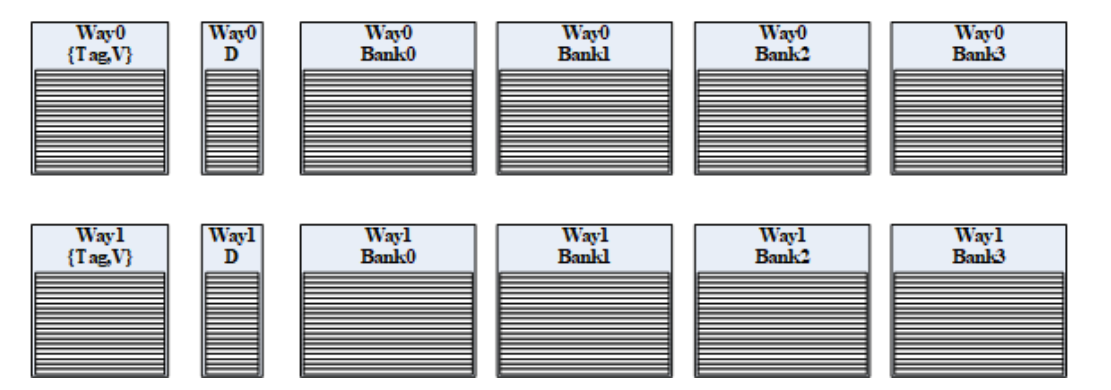
\includegraphics[width=0.8\textwidth]{fig/fig1.png}
        \caption{Cache逻辑组织结构}
        \label{fig:1}
    \end{figure}
    \begin{enumerate}
        \item data\_bank表
\begin{lstlisting}[language=verilog]
generate
for (i = 0; i < 4; i = i + 1)begin: data_way0
    data_bank_ram data_way0(
        .clka   (clk),
        .wea    (data_way0_wen[i]),   
        .addra  (data_way0_index[i]),
        .dina   (data_way0_wdata),
        .douta  (way0_data[i])  
    );
end
endgenerate
\end{lstlisting}
        一个Cache行有16个字节,分为4个data\_bank表。
        
        每一路的data\_bank表为一个RAM 256 * 32(深度*宽度)。

        \item tag,v表
\begin{lstlisting}[language=verilog]
    tagv_ram tagv_ram_way0 (
        .clka   (clk), 
        .wea    (tagv_way0_wen),
        .addra  (tagv_way0_index),
        .dina   ({tagv_way0_wdata}),
        .douta  ({way0_tag,way0_v})
    );
\end{lstlisting}    
        每个Cache行有一个tag和v域,表示该行是否有效和该行的在主存中的地址。

        由于所有Cache操作对tag和v的操作是完全一致的,所以,
        tag和v合并在一起存储,tag占高位,v占低位。
        
        每一路的tagv表用一个RAM 256 * 21(深度*宽度)存储。
        \item d表
    \begin{lstlisting}[language=verilog]
        d_regfile d_way0(
            .clk        (clk),
            .resetn     (resetn),
            .addr       (d_way0_index),
            .wen        (d_way0_wen),
            .wdata      (d_way0_wdata),
            .rdata      (way0_d)
        );   
    \end{lstlisting}
        每个Cache行有一个d域,表示该行的脏位,由于每行只有一个脏位,所以用regfile存储。

        每一路的d表用256个1位的寄存器堆存储。
    \end{enumerate}
    \item Cache的内部的控制逻辑设计
    \item 
    Cache 的控制包括两个状态机,主状态机和write buffer状态机。
    \begin{figure}[H]
        \centering
        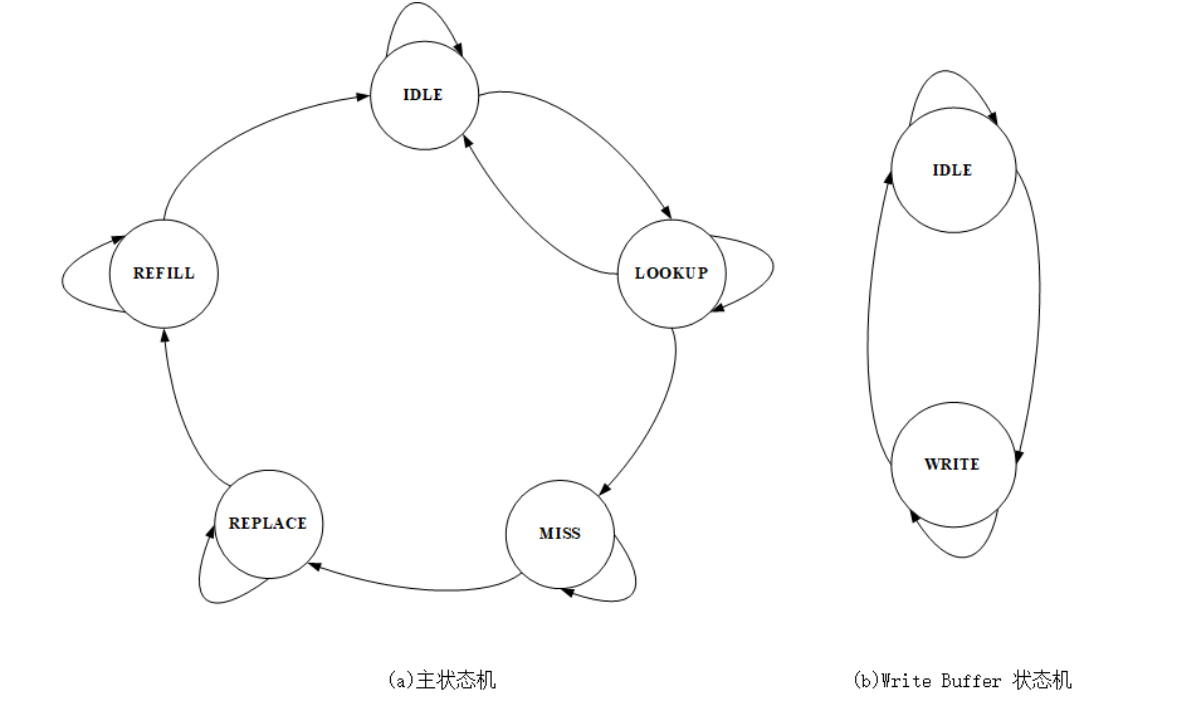
\includegraphics[width=0.8\textwidth]{fig/fig2.png}
        \caption{Cache的状态机}
        \label{fig:2}
    \end{figure}    
        
        主状态机包括5个状态,idle,lookup, miss, replace, refill。

        \begin{enumerate}
            \item idle状态
            
            在idle状态下,Cache等待外部的请求,当有请求到来,且与Cache中的Hit write不冲突时,用组合逻辑拉高addr\_ok信号,
            并在下一拍Cache进入lookup状态。
 \begin{lstlisting}[language=verilog]
assign addr_ok =    main_current_state == LOOKUP & cache_hit & ~hit_write_conflict
                    |main_current_state == IDLE & ~hit_write_conflict;
 \end{lstlisting}
 同时,将请求信息中的index通过组合逻辑,送到Cache进行查询,将两路的对应的Cache行的数据(tag, v, data)在下一拍读出来。

            并且,在request buffer中存储请求的相关信息。

\begin{lstlisting}[language=verilog]
// requeset buffer,存储接受到的请求信息
always @(posedge clk)begin
    if(~resetn) begin
        req_buffer_op <=       1'b0;
        req_buffer_index <=    8'b0;
        req_buffer_tag <=      20'b0;
        req_buffer_offset <=   4'b0;
        req_buffer_wstrb <=    4'b0;
        req_buffer_wdata <=    32'b0;
        req_buffer_type  =     1'b0;
    end
    else if(addr_ok & valid)begin      // next_state == LOOKUP,存储请求信息
        req_buffer_op <=       op;
        req_buffer_index <=    index;
        req_buffer_tag <=      tag;
        req_buffer_offset <=   offset;
        req_buffer_wstrb <=    wstrb;
        req_buffer_wdata <=    wdata;
        req_buffer_type  <=    type;       
    end
end
\end{lstlisting}
\item lookup状态

根据Cache的读出的两行的tag信息,与锁存在request buffer中的请求信息进行比较,如果有Hit,Cache进入idle状态,写操作将数据传给write buffer,
读操作直接返回Cache命中的数据。

否则进入miss状态。
\begin{lstlisting}[language=verilog]
// 请求的tag和Cache返回的tag比较,判断是否命中
    assign way0_hit = way0_v && (way0_tag == req_buffer_tag);
    assign way1_hit = way1_v && (way1_tag == req_buffer_tag);
    assign cache_hit = (way0_hit || way1_hit) && req_buffer_type;
\end{lstlisting}
为了在连续的cache命中时,保证ipc为1,则
如果在lookup命中,且接受到流水线的有效的访存请求,则直接在当前lookup状态下,向cache的发起对下一个请求的查询,将对应的Cache行的数据(tag, v, data)在下一拍读出来
,并在下一拍直接进入lookup状态,进行比较。

\begin{figure}[H]
    \centering
    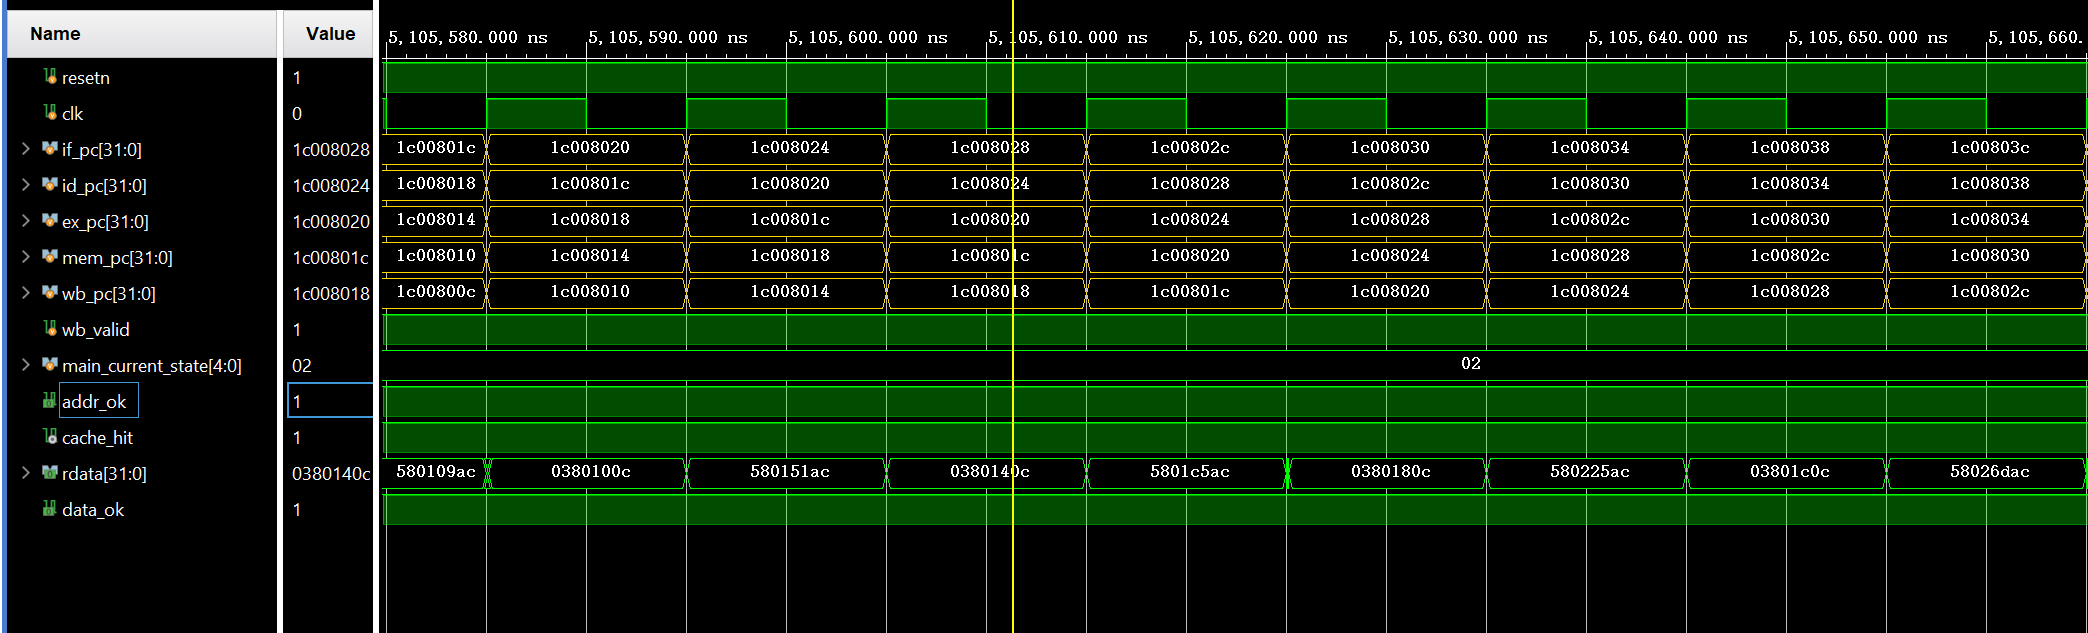
\includegraphics[width=0.8\textwidth]{fig/fig4.png}
    \caption{连续cache命中时的状态机}
    \label{fig:4}
\end{figure}
如图\ref{fig:4}
所示,当连续发生命中的时候,Cache的状态机不会进入idle状态,而是一直处于lookup状态,在当前的lookup状态对cache发起对下一个请求的查询。

\item miss状态

在miss状态下,等待AXI总线模块返回的wr\_rdy信号,当wr\_rdy信号为1时,Cache进入replace状态。
\begin{lstlisting}[language=verilog]
always @(*) begin
    case (main_current_state)
    MISS:
    if(~wr_rdy)         // 等待AXI总线模块返回的wr_rdy信号
        main_next_state = MISS;
    else
        main_next_state = REPLACE;
    endcase
end
\end{lstlisting}
\item replace状态

在replace状态的第一拍,如果需要,向AXI发起写请求,将替换出的Cache行写回主存。

同时,向AXI发起对Cache缺失的行的读请求。并且在读请求被接受后,Cache进入refill状态。
\begin{lstlisting}[language=verilog]
    //  在replace状态的第一拍,向AXI发起写请求
    assign wr_req =     first_clk_of_replace & replace_d & replace_v;
    assign wr_data =    replace_data;
    assign wr_addr =    {replace_tag, req_buffer_index, 4'b0};
    assign wr_type =    3'b100;
    assign wr_wstrb =    4'b1111;
    // 同时,向AXI发起对Cache缺失的行的读请求
    assign rd_req =     main_current_state == REPLACE;    // next_state == replace
    assign rd_addr =    {req_buffer_tag, req_buffer_index, 4'b0};
    assign rd_type =    3'b100;
\end{lstlisting}


\item refill状态

接受AXI返回的数据,将数据写入Cache中,在接受到最后一个数据后,Cache进入idle状态。
\begin{lstlisting}[language=verilog]
    always @(*) begin
        case (main_current_state)
        REFILL:
        if(ret_valid & ret_last)
            main_next_state = IDLE;
        else
            main_next_state = REFILL;
        endcase
    end
    \end{lstlisting}
如果是读请求,等到返回cpu请求的数据时(即miss\_buffer\_cnt == req\_buffer\_offset[3:2])
,即可拉高data\_ok信号,将数据传给cpu。不必等到Cache进入idle状态。
\begin{lstlisting}[language=verilog]
// 读请求,等到返回cpu请求的数据时,即可向cpu返回data_ok信号,并将数据传给cpu
assign data_ok =    (main_current_state == REFILL & ret_valid 
                    & miss_buffer_cnt == req_buffer_offset[3:2] & ~req_buffer_op)
                    |...;
\end{lstlisting}
\end{enumerate}
    
\end{enumerate}
$\bullet$
\textbf{在CPU中集成ICache}。

以tlb地址映射为例,如下图所示:
\begin{figure}[H]
    \centering
    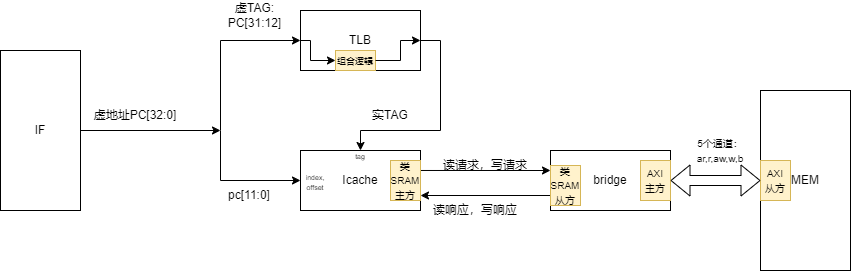
\includegraphics[width=\textwidth]{fig/fig3.png}
    \caption{ICache集成在CPU中示意图}
    \label{fig:3}
\end{figure}
\begin{enumerate}
    \item ICache与CPU的接口设计
    
由于Cache采用的是“虚Index实Tag”的方式,所以当cpu取指的时候,把虚拟地址的Index直接传递给Cache,Cache便开始根据虚拟地址的Index进行查询,

同时,将虚拟地址传递给虚实地址转换单元,它能通过组合逻辑在同一拍,将虚拟地址转换为物理地址的TAG,并传递给Cache。

上述方式使得Cache和TLB查询能并行执行,提高了效率。

    \item ICache与转接桥的接口设计
    
    Icache将访存请求发送到转接桥,转接桥将类sram的访存请求转换为AXI总线的访存请求,并且如果是多个字的访存请求,采用突发 burst 的方式。

    以写通道的burst控制为例,
    \begin{lstlisting}[language=verilog]
assign awlen =      awtype_reg == 3'b100 ? 8'd3 : 8'd0; // 如果是写整个cache行,burst长度为3
assign awsize =     3'b010; // 每拍发送一个字
assign awburst =    2'b01;  // 地址增加突发
assign wlast =      awtype_reg == 3'b100 ?wdata_cnt == 2'b11    // 最后一个字,拉高wlast
                    :1'b1;

always @(posedge clk)begin
    if(~resetn)begin
        wdata_cnt <= 2'b0;
    end
    else if(aw_current_state == AW_SEND_DATA && wready)begin
        wdata_cnt <= wdata_cnt + 1;
    end
end
    \end{lstlisting}

\end{enumerate}

\noindent
$\bullet$
\textbf{在CPU中集成DCache}。

与ICache集成在CPU中的结构类似,区别主要在于DCache与bridge之间的写请求和写响应是由意义的,而在ICache中因为不会有写操作因此icache模块写请求和写响应相关的信号无意义。

\begin{enumerate}
    \item DCache与CPU的接口设计

    Dcache的接口接法与Icache类似,输入信号主要来自于EX模块,输出信号中的地址OK信号发送给EX模块,数据OK信号发送给MEM模块。Dcache同样采用“虚Index实Tag”的方式。

    \item DCache与转接桥的接口设计

    与ICache相比,与转接桥相连的写请求与写响应端口不能再无视了。

    从DCache中连接至转接桥的wr\_req, wr\_type, wr\_addr, wr\_data, wr\_wstrb均在cache模块中赋值后发送。

    \begin{lstlisting}[language=verilog]
    assign wr_req =     first_clk_of_replace & (req_buffer_type ? (replace_d & replace_v)
                                            : req_buffer_op);   // non-cache write
    assign wr_data =    req_buffer_type ? replace_data : {4{req_buffer_wdata}};
    assign wr_addr =    req_buffer_type ? {replace_tag, req_buffer_index, 4'b0} 
                                        : {req_buffer_tag, req_buffer_index, req_buffer_offset};
    assign wr_type =    req_buffer_type ? 3'b100 : 3'b010;
    assign wr_wstrb =   req_buffer_type ? 4'b1111 : req_buffer_wstrb;
    \end{lstlisting}
    
    传给DCache的wr\_rdy和wr\_bvalid信号分别连接至转接桥的data\_sram\_wr\_addr\_ok和data\_sram\_wr\_data\_ok。

    \begin{lstlisting}[language=verilog]
assign data_sram_wr_addr_ok = aw_current_state == AW_WAIT;
assign data_sram_wr_data_ok = b_current_state == B_WAIT;
    \end{lstlisting}

    \item 非缓存

    在cache模块中添加一个一位宽的表示是否可缓存的变量type。

    icache和dcache的type的值均在csrfile.v内做判断。直接地址翻译模式下存储类型由CRMD的DATF和DATM域决定,直接映射地址翻译模式下由命中窗口的MAT域决定,页表映射地址翻译模式下由所用页表项的MAT域决定。

    \begin{lstlisting}[language=verilog]
    assign inst_type = (~csr_crmd_pg) ? (csr_crmd_datf==2'b01) :
                       hit_dmw0 ? (csr_dmw0_mat==2'b01) :
                       hit_dmw1 ? (csr_dmw1_mat==2'b01) :
                       s0_mat;
    assign data_type = (~csr_crmd_pg) ? (csr_crmd_datm==2'b01) :
                       hit_dmw0 ? (csr_dmw0_mat==2'b01) :
                       hit_dmw1 ? (csr_dmw1_mat==2'b01) :
                       s1_mat;
    \end{lstlisting}

    之后再根据传进cache模块的type变量对cache模块做修改。确保发生非缓存时不对cache缓存做任何修改。

    以非缓存的load指令为例,确保LOOKUP状态不看比较结果直接进入MISS状态,且不向Cache发送读操作,也不产生对外的替换写。

    \begin{lstlisting}[language=verilog]
    assign cache_hit = (way0_hit || way1_hit) && req_buffer_type;
    assign data_ok =    (main_current_state == REFILL & ret_valid & (((miss_buffer_cnt == req_buffer_offset[3:2]) & req_buffer_type) | ~req_buffer_type) & ~req_buffer_op)         // read miss
                        |(main_current_state == LOOKUP & (cache_hit | req_buffer_op));             // hit or write
            assign data_way0_wen[i] =    (wr_current_state == WR_WRITE & w_buffer_way == 0 & w_buffer_bank == i)? w_buffer_wstrb
                                        :(main_current_state == REFILL & replace_way ==0 & ret_valid & miss_buffer_cnt == i & req_buffer_type) ? 4'b1111
                                        :4'b0000;
    \end{lstlisting}
    
\end{enumerate}

\noindent
$\bullet$
\textbf{cacop指令的添加}。
\begin{enumerate}
    \item CACOP指令基本数据通路
    
    首先需要添加cacop指令的译码信号,然后在流水线中搭建数据通路
    \begin{lstlisting}[language=verilog]
    wire inst_cacop;
    assign inst_cacop = op_31_26_d[6'h01] &op_25_22_d[4'h8];
    assign cacop_code = inst_ID[4:0]; //cacop指令码传入两个Cache
    assign icacop =inst_cacop&cacop_code[2:0]==3'b000;//该信号传入ICache
    assign dcacop =ex_inst_cacop & ex_cacop_code[2:0]==3'b001;//该信号传入DCache
    \end{lstlisting}
    \item Cache模块中对CACOP指令的实现
    
    的cacop指令都可能涉及对于tagv的读写,以way0为例,当为初始化指令时,将指定Cache行的tagv写为0;当为一致化指令时,将指定Cache行的tag保留,将valid
    位置为0。详细代码如下:
    \begin{lstlisting}[language=verilog]
        // tag, v table
        assign tagv_way0_index =    (main_current_state == LOOKUP || main_current_state == IDLE) ? index   // look up
                                    :req_buffer_index;      // replace and refill;
        assign tagv_way0_wen =  main_current_state == REFILL & replace_way == 0 & ret_valid & ret_last & req_buffer_type
                                | cacop & offset[0]== 0 & code[4:3] != 2'b10 
                                | cacop_wr_tagv & way0_v & (way0_tag == tag) & req_buffer_type & code[4:3]==2'b10;     
    
        assign tagv_way0_wdata = {req_buffer_tag, 1'b1} & {21{ret_valid & ret_last & replace_way == 0 & req_buffer_type}}
                                | {reg_tagv_dcacop[20:1], 1'b0} & {21{cacop & offset[0] == 0 & (code[4:3] == 2'b01 | code[4:3] == 2'b10)}}
                                | {21'b0} & {21{cacop & offset[0] == 0 & code[4:3] == 2'b00}};
    \end{lstlisting}

    此外,ICache没有其他操作,但DCache可能涉及到写内存操作,此时需要一个标志信号来记录本指令是否
需要写内存,代码如下:
    \begin{lstlisting}[language=verilog]
        wire   cache_write_new;
        assign cache_write_new = (offset[0] ? way1_d : way0_d) & (offset[0] ? {way1_tag,way1_v} : {way0_tag,way0_v} ) & cacop & code[4:3] == 2'b01
                                | way0_d & way0_v & cacop & code[4:3] == 2'b10 & way0_hit 
                                | way1_d & way1_v & cacop & code[4:3] == 2'b10 & way1_hit;
        
        reg cache_write_reg;
        always @(posedge clk) begin
            if (!resetn) begin
                cache_write_reg <= 1'b0;
            end
            else if (cache_write_new) begin
                 cache_write_reg <= 1'b1;
            end
            else if (~cacop) begin
                cache_write_reg <= 1'b0;
            end
        end
    
        reg cacop_hit;
        always @(posedge clk) begin
            if (!resetn) begin
                cacop_hit <= 1'b0;
            end
            else if (cacop & cache_write) begin
                cacop_hit <= 1'b1;
            end
            else if (~cacop) begin
                cacop_hit <= 1'b0;
            end
        end
    
        assign cache_write = (cache_write_reg | cache_write_new) & cacop & (code[4:3] == 2'b01 | code[4:3] == 2'b10 & (cacop_hit | cache_hit));    
    \end{lstlisting}
    
    使用该信号控制状态机,使其进入MISS状态
    \begin{lstlisting}[language=verilog]
        LOOKUP:
        if(cache_hit & (~valid | ~addr_ok) & ~cache_write)
            main_next_state = IDLE;
        else if(~cache_hit & ~cache_write)
            main_next_state = MISS;
        else
            main_next_state = LOOKUP;

    MISS:
        if(~wr_rdy)
            main_next_state = MISS;
        else
            main_next_state = REPLACE;
    \end{lstlisting}

    在MISS状态下,其向AXI总线桥发出相应的访存信号,代码如下:
    \begin{lstlisting}[language=verilog]
        assign wr_req =     first_clk_of_replace & (req_buffer_type ? (replace_d & replace_v)
        : (cacop & code[4:3] == 2'b01 & (req_buffer_offset[0] ? way1_d:way0_d) & reg_tagv_dcacop[0] |cacop & code[4:3] == 2'b10 & cache_write) ? 1
        : req_buffer_op);   // non-cache write
        assign wr_data =    req_buffer_type | cacop  ? replace_data_final : {4{req_buffer_wdata}};
        assign wr_addr =    req_buffer_type & ~cacop ? {replace_tag, req_buffer_index, 4'b0} 
        : cacop & code[4:3]==2'b01 ? {reg_tagv_dcacop[20:1],req_buffer_index,req_buffer_offset[3:1],1'b0}
        : {req_buffer_tag, req_buffer_index, req_buffer_offset};


    assign wr_type =    req_buffer_type | cacop ? 3'b100 : 3'b010;
    assign wr_wstrb =   req_buffer_type | cacop ? 4'b1111 : req_buffer_wstrb;
    \end{lstlisting}

    其中,reg_tagv_dcacop是用来寄存即将写入dacache中tagv的寄存器
    \begin{lstlisting}[language=verilog]
        reg [20:0] reg_tagv_dcacop;
        always @(posedge clk) begin
            if (!resetn) begin
            reg_tagv_dcacop <= 20'b0;
            end
            else if (~(|reg_tagv_dcacop) & cacop & code[4:3] == 2'b01) begin
                reg_tagv_dcacop <= offset[0] ?  {way1_tag,way1_v} : {way0_tag,way0_v};
            end
            else if (~(|reg_tagv_dcacop) & cacop & code[4:3] == 2'b10 & way0_hit) begin
                reg_tagv_dcacop <= {way0_tag,way0_v};
            end
            else if (~(|reg_tagv_dcacop) & cacop & code[4:3] == 2'b10 & way1_hit) begin
                reg_tagv_dcacop <= {way1_tag,way1_v};
            end
            else if((|reg_tagv_dcacop) & ~cacop) begin
                reg_tagv_dcacop <= 20'b0;
            end 
        end
    \end{lstlisting}
    \item CPU中ICache对CACOP指令的实现
    
    将ICache的cacop执行位于ID阶段,下一条指令取值之前。ICache的cacop指令信号需要挤占ICache取指信号的通路,然后
    在if模块添加新的通路,代码如下:
    \begin{lstlisting}[language=verilog]
        assign inst_vindex = inst_sram_addr[11: 4] & {8{~icacop | cacop_code[4:3]==2'b10 | icacop_complete}}
                    | icacop_addr[11: 4] & {8{icacop & ~icacop_complete & cacop_code[4:3]!=2'b10}};

        assign inst_voffset =inst_sram_addr[ 3: 0] & {4{~icacop | cacop_code[4:3]==2'b10 | icacop_complete}}
                    | icacop_addr[ 3: 0] & {4{icacop & ~icacop_complete & cacop_code[4:3]!=2'b10}};
                    assign pre_pc_pa =          (!csr_crmd_pg | inst_cacop & cacop_code[4:3] == 2'b00 | inst_cacop & cacop_code[4:3] == 2'b01) ? pre_pc            // direct translate
                    :pre_pc_map;                    // enable mapping
                
                assign hit_dmw0 =           csr_dmw0_plv_met & csr_dmw0_vseg == pre_pc[31:29];
                assign hit_dmw1 =           csr_dmw1_plv_met & csr_dmw1_vseg == pre_pc[31:29];

                assign pre_pc_map =         hit_dmw0 ? {csr_dmw0_pseg, pre_pc[28:0]}         // dierct map windows 0
                    :hit_dmw1? {csr_dmw1_pseg, pre_pc[28:0]}         // direct map windows 1
                    :(s0_ps == 6'b010101) ? {s0_ppn[19:9], icacop_vaddr[20:0]}   // tlb map: ps 4Mb
                    :{s0_ppn,icacop_vaddr[11:0]};                             // tlb map : ps 4kb

    \end{lstlisting}

    其中的icacop_complete信号,用来标记ICache的cacop指令是否执行完毕,这是因为op为10时,需要两个周期才能完成,op不为10时需一个周期完成。其代码如下
    \begin{lstlisting}[language=verilog]
        always @(posedge clk) begin
    if (~resetn) begin
        icacop_complete <= 1'b1;
    end
    else if (icacop & cacop_code[4:3] != 2'b10) begin
        icacop_complete <= 1'b1;
    end
    else if (icacop_next & cacop_code[4:3] == 2'b10) begin
        icacop_complete <= 1'b1;
    end
    else  
        icacop_complete <= 1'b0;
    end
    \end{lstlisting}

    当op为10时,需要将cacop指令的虚拟地址s0_vppn, s0_va_bit12传入tlb,代码如下:
    \begin{lstlisting}[language=verilog]
        assign icacop_vaddr = pre_pc & {32{~icacop| cacop_code[4:3]!=2'b10|icacop_complete}}
        | icacop_addr&{32{icacop & ~icacop_complete &cacop_code[4:3]==2'b10}};
        assign {s0_vppn, s0_va_bit12} = icacop_vaddr[31:12];// output to tlb
    \end{lstlisting}
    \item CPU中DCache对CACOP指令的实现
    
    dcache的主要操作与icache相类似,此处不再赘述。

    \begin{lstlisting}[language=verilog]
        assign sram_addr_pa =       (!csr_crmd_pg | ex_cacop & ex_cacop_code == 5'b00001 | ex_cacop & ex_cacop_code == 5'b01001) ? ex_alu_result    // direct translate
        :  sram_addr_map  ;                 // enable mapping
    
        assign hit_dmw0 =           csr_dmw0_plv_met & csr_dmw0_vseg == ex_alu_result[31:29] & ~(dcacop & ex_cacop_code[4:3] != 2'b10);
        assign hit_dmw1 =           csr_dmw1_plv_met & csr_dmw1_vseg == ex_alu_result[31:29] & !hit_dmw0 & ~(dcacop & ex_cacop_code[4:3] != 2'b10);

        assign sram_addr_map =       hit_dmw0 ? {csr_dmw0_pseg, ex_alu_result[28:0]}         // dierct map windows 0
                :hit_dmw1? {csr_dmw1_pseg, ex_alu_result[28:0]}         // direct map windows 1
                :(s1_ps == 6'b010101) ? {s1_ppn[19:9], ex_alu_result[20:0]}   // tlb map: ps 4Mb
                :{s1_ppn,ex_alu_result[11:0]};                             // tlb map : ps 4kb
//
wire dcacop;
assign dcacop = ex_cacop & (ex_cacop_code[2:0] == 3'b001);
    \end{lstlisting}
\end{enumerate}



\section{实验过程中遇到的问题、对问题的思考过程及解决方法(比如RTL代码中出现的逻辑bug,逻辑仿真和FPGA调试过程中的难点等)}

\noindent
$\bullet$
\textbf{Cache模块时向cpu的data\_ok信号设置}。
最初,由于下意识认为cpu是串行工作,所以不论是读还是写,都等到Cache的状态机走完一圈后,返回idle状态,再向cpu返回data\_ok信号。

但是,实际上,流水线和Cache是并行工作的,所以只要Cache可以返回读数据或者接受了写数据,就可以向cpu返回data\_ok信号,让流水线可以继续工作。

至于要保证Cache采用
阻塞式设计(即一旦发生缺失,Cache就不再接受新的请求,直到缺失的数据返回),需要用addr\_ok信号来控制,等到Cache的状态机走完一圈后,接受完缺失的数据,再接受新的请求。

\begin{lstlisting}[language=verilog]
assign addr_ok =    main_current_state == LOOKUP & cache_hit & ~hit_write_conflict      // 如果发生数据缺失,Cache拉低add_ok,不接受新的请求
                    |main_current_state == IDLE & ~hit_write_conflict;
assign data_ok =    
(main_current_state == REFILL & ret_valid & miss_buffer_cnt == req_buffer_offset[3:2] & ~req_buffer_op) 
 // 读缺失时,在refill状态下,等到返回cpu请求的数据时,即可向cpu返回data_ok信号
|(main_current_state == LOOKUP & (cache_hit | req_buffer_op)); 
// 写操作,不管是否命中,都将向cpu返回data_ok信号,表示请求已经接受
\end{lstlisting}


      
\vspace{1ex}

\section{小组成员分工合作情况}
王敬华负责cacop指令的实现。

李霄宇负责集成dCache到cpu中,非缓存的添加。

艾华春负责Cache模块设计,集成iCache到cpu中。

实验报告为根据每人负责代码的部分,写相应部分的报告。
\end{document}